%%%%%%%%%%%%%%%%%%%%%%%%%%%%%%%%%%%%%%%%%
% Short Sectioned Assignment
% LaTeX Template
% Version 1.0 (5/5/12)
%
% This template has been downloaded from:
% http://www.LaTeXTemplates.com
%
% Original author:
% Frits Wenneker (http://www.howtotex.com)
%
% License:
% CC BY-NC-SA 3.0 (http://creativecommons.org/licenses/by-nc-sa/3.0/)
%
%%%%%%%%%%%%%%%%%%%%%%%%%%%%%%%%%%%%%%%%%

%----------------------------------------------------------------------------------------
%	PACKAGES AND OTHER DOCUMENT CONFIGURATIONS
%----------------------------------------------------------------------------------------

\documentclass[paper=a4, fontsize=11pt]{scrartcl} % A4 paper and 11pt font size 

\usepackage[T1]{fontenc} % Use 8-bit encoding that has 256 glyphs
\usepackage[english]{babel} % English language/hyphenation
\usepackage{amsmath,amsfonts,amsthm} % Math packages

\usepackage{sectsty} % Allows customizing section commands
%\allsectionsfont{\centering \normalfont\scshape} % Make all sections centered, the default font and small caps

\usepackage{fancyhdr} % Custom headers and footers
\pagestyle{fancyplain} % Makes all pages in the document conform to the custom headers and footers
\fancyhead{} % No page header - if you want one, create it in the same way as the footers below
\fancyfoot[L]{} % Empty left footer
\fancyfoot[C]{} % Empty center footer
\fancyfoot[R]{\thepage} % Page numbering for right footer
\renewcommand{\headrulewidth}{0pt} % Remove header underlines
\renewcommand{\footrulewidth}{0pt} % Remove footer underlines
\setlength{\headheight}{13.6pt} % Customize the height of the header

\numberwithin{equation}{section} % Number equations within sections (i.e. 1.1, 1.2, 2.1, 2.2 instead of 1, 2, 3, 4)
\numberwithin{figure}{section} % Number figures within sections (i.e. 1.1, 1.2, 2.1, 2.2 instead of 1, 2, 3, 4)
\numberwithin{table}{section} % Number tables within sections (i.e. 1.1, 1.2, 2.1, 2.2 instead of 1, 2, 3, 4)

\setlength\parindent{0pt} % Removes all indentation from paragraphs - comment this line for an assignment with lots of text

\usepackage{bbm}
\usepackage{graphicx}
\usepackage{xcolor} % For color
\usepackage{subcaption}
\usepackage{booktabs}

\usepackage{tikz} % For graphs
\usetikzlibrary{positioning}
\usetikzlibrary{calc}

\usepackage{enumerate} % For lettered enumeration
%----------------------------------------------------------------------------------------
%	TITLE SECTION
%----------------------------------------------------------------------------------------

\newcommand{\horrule}[1]{\rule{\linewidth}{#1}} % Create horizontal rule command with 1 argument of height

\title{	
\normalfont \normalsize 
\horrule{0.5pt} \\[0.4cm] % Thin top horizontal rule
\huge Assignment Four \\ % The assignment title
\horrule{2pt} \\[0.5cm] % Thick bottom horizontal rule
}

\author{
	Matthew C.~Scicluna\\
	D\'epartement d'Informatique et de Recherche Op\'erationnelle\\
	Universit\'e de Montr\'eal\\
	Montr\'eal, QC H3T 1J4 \\
	\texttt{matthew.scicluna@umontreal.ca}
}


\date{\normalsize\today} % Today's date or a custom date

\begin{document}

\maketitle % Print the title

%----------------------------------------------------------------------------------------
%	PROBLEM 1
%----------------------------------------------------------------------------------------

\section{Entropy and Mutual Information}
	Let \(X\) be a discrete random variable on a finite space \(\mathcal{X}\) with \(|\mathcal{X}| = k\).
\begin{enumerate} 
	\item\begin{enumerate}[(a)]
		\item Prove that the entropy \(H(X)\ge0\), with equality only when X is a constant.
		
		PROOF: WLOG we can assume that \(p(x)>0 \ \forall x\in\mathcal{X}\), (using that \(0\cdot log0 = 0\)). We have that \(H(X) = -\sum_{x} p(x)logp(x) = \sum_{x} p(x)logp(x)^{-1}\ge0\), since \(p(x)>0\) and \(p(x)^{-1} \ge 1\). If \(H(X)=0\) then \(\exists \alpha\) such that \(p(\alpha)^{-1}=1 \Rightarrow p(\alpha)=1\). Hence \(X\) must be a constant, as needed.
		\item Let \(X \sim p\) and \(q\) be the Uniform distribution on \(\mathcal{X}\). What is the relation between \(D(p||q)\) and \(H(X)\).
		
		CLAIM: \(D(p||q) = -H(X) + logk\)
		
		PROOF: 
		\begin{align*}
		D(p||q)&=\sum_{x}p(x)log\frac{p(x)}{q(x)}\\
		&=\sum_{x}p(x)logp(x)-\sum_xp(x)logq(x)\\
		&= -H(X) + \sum_xp(x)logk \\
		&= -H(x) + logk
		\end{align*}
		\item An upper bound for \(H(X)\) is \(logk\) since \(H(X)=logk-D(p||q) \Rightarrow H(X) \le logk \).
		\end{enumerate}
		We consider a pair of discrete random variables \((X_1,X_2)\) defined over the finite set \(\mathcal{X}_1\times\mathcal{X}_2\).
		Let \(p_{1,2}\), \(p_1\) and \(p_2\) denote respectively the joint distribution, the marginal distribution of \(X_1\) and the marginal distribution of \(X_2\). Define the mutual information as:
		\begin{align*}
		I(X_1,X_2)=\sum_{(x_1,x_2)\in\mathcal{X}_1\times\mathcal{X}_2}p_{1,2}(x_1,x_2)log\frac{p_{1,2}(x_1,x_2)}{p_1(x_1)p_2(x_2)}
		\end{align*}
		We again assume WLOG that \(p(x_1,x_2)>0 \ \forall (x_1,x_2)\in\mathcal{X}_1\times\mathcal{X}_2\)
		
	\item\begin{enumerate}[(a)]
		\item CLAIM: \(I(X_1,X_2)\ge 0\)
		
		PROOF: Notice that \(I(X_1,X_2) = D(p_{1,2}||p_1p_2) \ge 0\) by the positiveness of \(D(\cdot||\cdot)\).
		
		\item We want to express  \(I(X_1,X_2)\) as a function of \(H(X_1), H(X_2)\) and \(H(X_1,X_2)\).
		\begin{align*}
		I(X_1,X_2) &= \sum_{(x_1,x_2)\in\mathcal{X}_1\times\mathcal{X}_2}p_{1,2}(x_1,x_2)log\frac{p_{1,2}(x_1,x_2)}{p_1(x_1)p_2(x_2)} \\
		&=\sum_{(x_1,x_2)\in\mathcal{X}_1\times\mathcal{X}_2}p_{1,2}(x_1,x_2)logp_{1,2}(x_1,x_2)-p_{1,2}(x_1,x_2)logp_1(x_1)p_2(x_2)\\
		&=-H(X_1,X_2) - \sum_{(x_1,x_2)\in\mathcal{X}_1\times\mathcal{X}_2}\bigg( p_1(x_1)p_2(x_2)logp_1(x_1) - p_1(x_1)p_2(x_2)logp_2(x_2) \bigg) \\
		&=-H(X_1,X_2) - \sum_{j=1}^{2}\sum_{(x_1,x_2)\in\mathcal{X}_1\times\mathcal{X}_2}p_1(x_1)p_2(x_2)logp_j(x_j)\\
		&= -H(X_1,X_2) -\sum_{j=1}^{2}\sum_{x_j\in\mathcal{X}_j}p_j(x_j)logp_j(x_j)\\
		&= -H(X_1,X_2) + H(X_1) + H(X_2)
		\end{align*}
		And so we can represent \(I(X_1,X_2)\) using \(H(X_1), H(X_2)\) and \(H(X_1,X_2)\), as needed.
		\item From the previous result we have that \(I(X_1,X_2)\ge0 \Rightarrow H(X_1) + H(X_2) \ge H(X_1,X_2) \), and so the maximal entropy of \((X_1,X_2)\) is \(H(X_1) + H(X_2)\). By definition this only occurs when \(I(X_1,X_2)=0\), which only occurs if
		\(p_{1,2}(x_1,x_2)=p_1(x_1)p_2(x_2) \ \forall x_1,x_2 \in \mathcal{X}_1\times\mathcal{X}_2\). This can be seen directly from the definition of \(I\) and using the strict positivity of \(p(x_1,x_2)\).
		\end{enumerate}
	\end{enumerate}

\newpage

\section{HMM -- Implementation}

We use an HMM model to account for the possible temporal structure of some data.
We consider the following HMM model: the chain \((z_t)_{t=1}^T\) has \(K=4\) possible states, with an initial
probability distribution \(\pi\in\Delta_4\) and a probability transition matrix \(A\in\mathbb{R}^{4\times4}\) where \(A_{ij} = p(z_t = i | z_{t-1} = j)\) and conditionally on the current state \(z_t\), we have observations obtained from Gaussian emission probabilities \(x_t |(z_t = k) \sim N(x_t |\mu_k , \Sigma_k )\).

\subsection{Fake Parameters Inference}
We computed the vectors \(\alpha(z_t)=p(z_t,x_{1:t})\) and \(\beta(z_t)=p(x_{(t+1):T} | z_t)\) on the test set from Assignment 3 using the following parameters: \(\pi_k = \frac{1}{4}\), \(A_{ii}=\frac{1}{2}\) and \(A_{ij}=\frac{1}{6}, i\ne j\), and \(\mu_k, \Sigma_k\) as defined in the homework. 
We used these to compute the posterior of the latent variable over time \(p(z_t \mid x_1, \cdots, x_T)\). We plotted the first 100 datapoints in figure 2.1.

\begin{figure}
	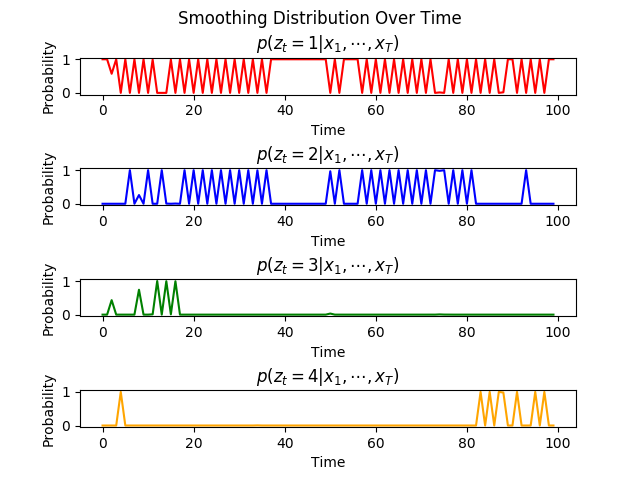
\includegraphics[width=.9\linewidth]{smoothing_dist.png}
	\caption{The smoothing distribution for the first 100 time points.}
\end{figure}

\subsection{M-Step Derivation}
We now derive the M-Step for the Hidden Markov Model. \\
Let \(\theta^{(s)} = (\pi^{(s)}, A^{(s)}, \mu_1^{(s)}, \cdots, \mu_K^{(s)}, \Sigma_1^{(s)}, \cdots,\Sigma_K^{(s)})\) be the ML parameters learned during step \(s\) of EM. Let \(\gamma_{tk}=P(z_t=k|x_{1:T})\) and \(\xi_{tlm}=P(z_t=l,z_{t+1}=m|x_{1:T})\) - which are the quantities that were computed in the E-Step using \(\theta^{(s)}\).
The Expected Complete Data Log-Likelihood (at step \(s+1\)) is:
\begin{equation}
Q(\theta, \theta^{(s)}) = \sum_{k=1}^K \gamma_{tk}log\pi_k + \sum_{t=1}^T\sum_{k=1}^K \gamma_{tk}P(\bar{x}_t|\mu_{k}, \Sigma_{k}) + \sum_{t=1}^{T-1} \sum_{l=1}^K\sum_{m=1}^K\xi_{tlm}logA_{lm}
\end{equation}

To solve for \(\pi_k\) we look for stationary points, subject to the constraint \(\sum_{k=1}^K\pi_k = 1\)

\begin{align}
&\frac{\partial}{\partial\pi_k} Q(\theta, \theta^{(s)}) - \lambda \left(\sum_{k=1}^K\pi_k - 1 \right) = \frac{\gamma_{1k}}{\pi_k}-\lambda = 0\\
&\Rightarrow \pi_k = \frac{\gamma_{1k}}{\lambda}
\end{align}
And using that \(\sum_{k=1}^K\pi_k = 1\) we have that:
\begin{align}
\pi_k^{(s+1)} = \frac{\gamma_{1k}}{\sum_{l=1}^K\gamma_{1l}}
\end{align}

To solve for \(A_{lm}\) we look for stationary points, subject to the constraint \(\sum_{l=1}^K A_{lm} = 1\)
\begin{align}
&\frac{\partial}{\partial A_{lm}} Q(\theta, \theta^{(s)}) - \lambda \left(\sum_{l=1}^K A_{lm} - 1 \right) = \sum_{t=1}^{T-1}\frac{\xi_{tlm}}{A_{lm}}-\lambda = 0\\
&\Rightarrow A_{lm} = \frac{\sum_{t=1}^{T-1}\xi_{tlm}}{\lambda}
\end{align}
And using that \(\sum_{l=1}^K A_{lm} = 1\) we have that:
\begin{align}
A_{lm}^{(s+1)} = \frac{\sum_{t=1}^{T-1}\xi_{tlm}}{\sum_{l=1}^K\sum_{t=1}^{T-1}\xi_{tlm}}
\end{align}

To solve for \(\mu_k\) we look for stationary points
\begin{align}
\frac{\partial}{\partial \mu_{k}} Q(\theta, \theta^{(s)}) &= \sum_{t=1}^{T}\frac{\partial}{\partial \mu_{k}}\frac{-\gamma_{tk}}{2}(\bar{x}_t-\mu_k)^T\Sigma_k^{-1}(\bar{x}_t-\mu_k) \\
&=\sum_{t=1}^{T}\frac{-\gamma_{tk}}{2}(\bar{x}_t-\mu_k)\Sigma_k^{-1}=0\\
&\Rightarrow \sum_{t=1}^{T-1}\gamma_{tk}(\bar{x}_t-\mu_k)=0\\
&\Rightarrow \mu_k^{(s+1)} = \frac{\sum_{t=1}^{T}\gamma_{tk}\bar{x}_t}{\sum_{t=1}^{T-1}\gamma_{tk}}
\end{align}

To solve for \(\Sigma_k\) we look for stationary points. As in assignment 1, we take the derivative w.r.t \(\Sigma^{-1}_k\)
\begin{align}
\frac{\partial}{\partial \Sigma^{-1}_{k}} Q(\theta, \theta^{(s)}) &= \sum_{t=1}^{T}\frac{\partial}{\partial \mu_{k}}\left(\frac{-\gamma_{tk}}{2}log|\Sigma_k| -\frac{\gamma_{tk}}{2}\left(\bar{x}_t-\mu_k^{(s+1)}\right)^T\Sigma_k^{-1}\left(\bar{x}_t-\mu_k^{(s+1)}\right)\right)
\end{align}

Differentiating the first term yields
\begin{align}
\frac{\partial}{\partial \Sigma^{-1}_{k}}\frac{-\gamma_{tk}}{2}log|\Sigma_k|
&=\frac{\partial}{\partial \Sigma^{-1}_{k}}\frac{\gamma_{tk}}{2}log|\Sigma^{-1}_k|\\
&=\frac{\gamma_{tk}}{2}\Sigma_k
\end{align}

Differentiating the second term yields
\begin{align}
&\frac{\partial}{\partial \Sigma^{-1}}\frac{\gamma_{tk}}{2}\left(\bar{x}_t-\mu_k^{(s+1)}\right)^T\Sigma_k^{-1}\left(\bar{x}_t-\mu_k^{(s+1)}\right)\\
&=\frac{\partial}{\partial \Sigma^{-1}}\frac{\gamma_{tk}}{2}tr\left(\left(\bar{x}_t-\mu_k^{(s+1)}\right)\left(\bar{x}_t-\mu_k^{(s+1)}\right)^T\Sigma_k^{-1}\right)\\
&= \frac{\gamma_{tk}}{2}\left(\bar{x}_t-\mu_k^{(s+1)}\right)\left(\bar{x}_t-\mu_k^{(s+1)}\right)^T
\end{align}
Where (2.15) and (2.16) come from results proved in class and on Homework 1. After substituting (2.14) and (2.17) into (2.12) and equating to 0 we have that:

\begin{align}
&\sum_{t=1}^{T}\gamma_{tk}\Sigma_k=\sum_{t=1}^{T}
\gamma_{tk}\left(\bar{x}_t-\mu_k^{(s+1)}\right)\left(\bar{x}_t-\mu_k^{(s+1)}\right)^T\\
&\Rightarrow \Sigma_k^{(s+1)} = \frac{\sum_{t=1}^{T}\gamma_{tk}(\bar{x}_t-\mu_k^{(s+1)})(\bar{x}_t-\mu_k^{(s+1)})^T}{\sum_{t=1}^{T}\gamma_{tk}}
\end{align}

\end{document}